\appendixpage
\section{The effect of discarding the first run}
\label{sec:effect-of-disregarding-the-first-run}
In performance benchmarking, particularly when using libraries like CBLAS, the first execution of a matrix multiplication algorithm often demonstrates significantly lower performance compared to subsequent runs. This reduction in performance is primarily due to overhead introduced by factors such as dynamic library loading and memory allocation, which can skew the results of the initial run. Figure \ref{fig:mflops-Basic-CBLAS-2nd-run} presents the results after discarding the first run for each matrix size, showing a more consistent and gradual increase in performance for CBLAS MM.


\begin{figure}[htbp]
    \centering
    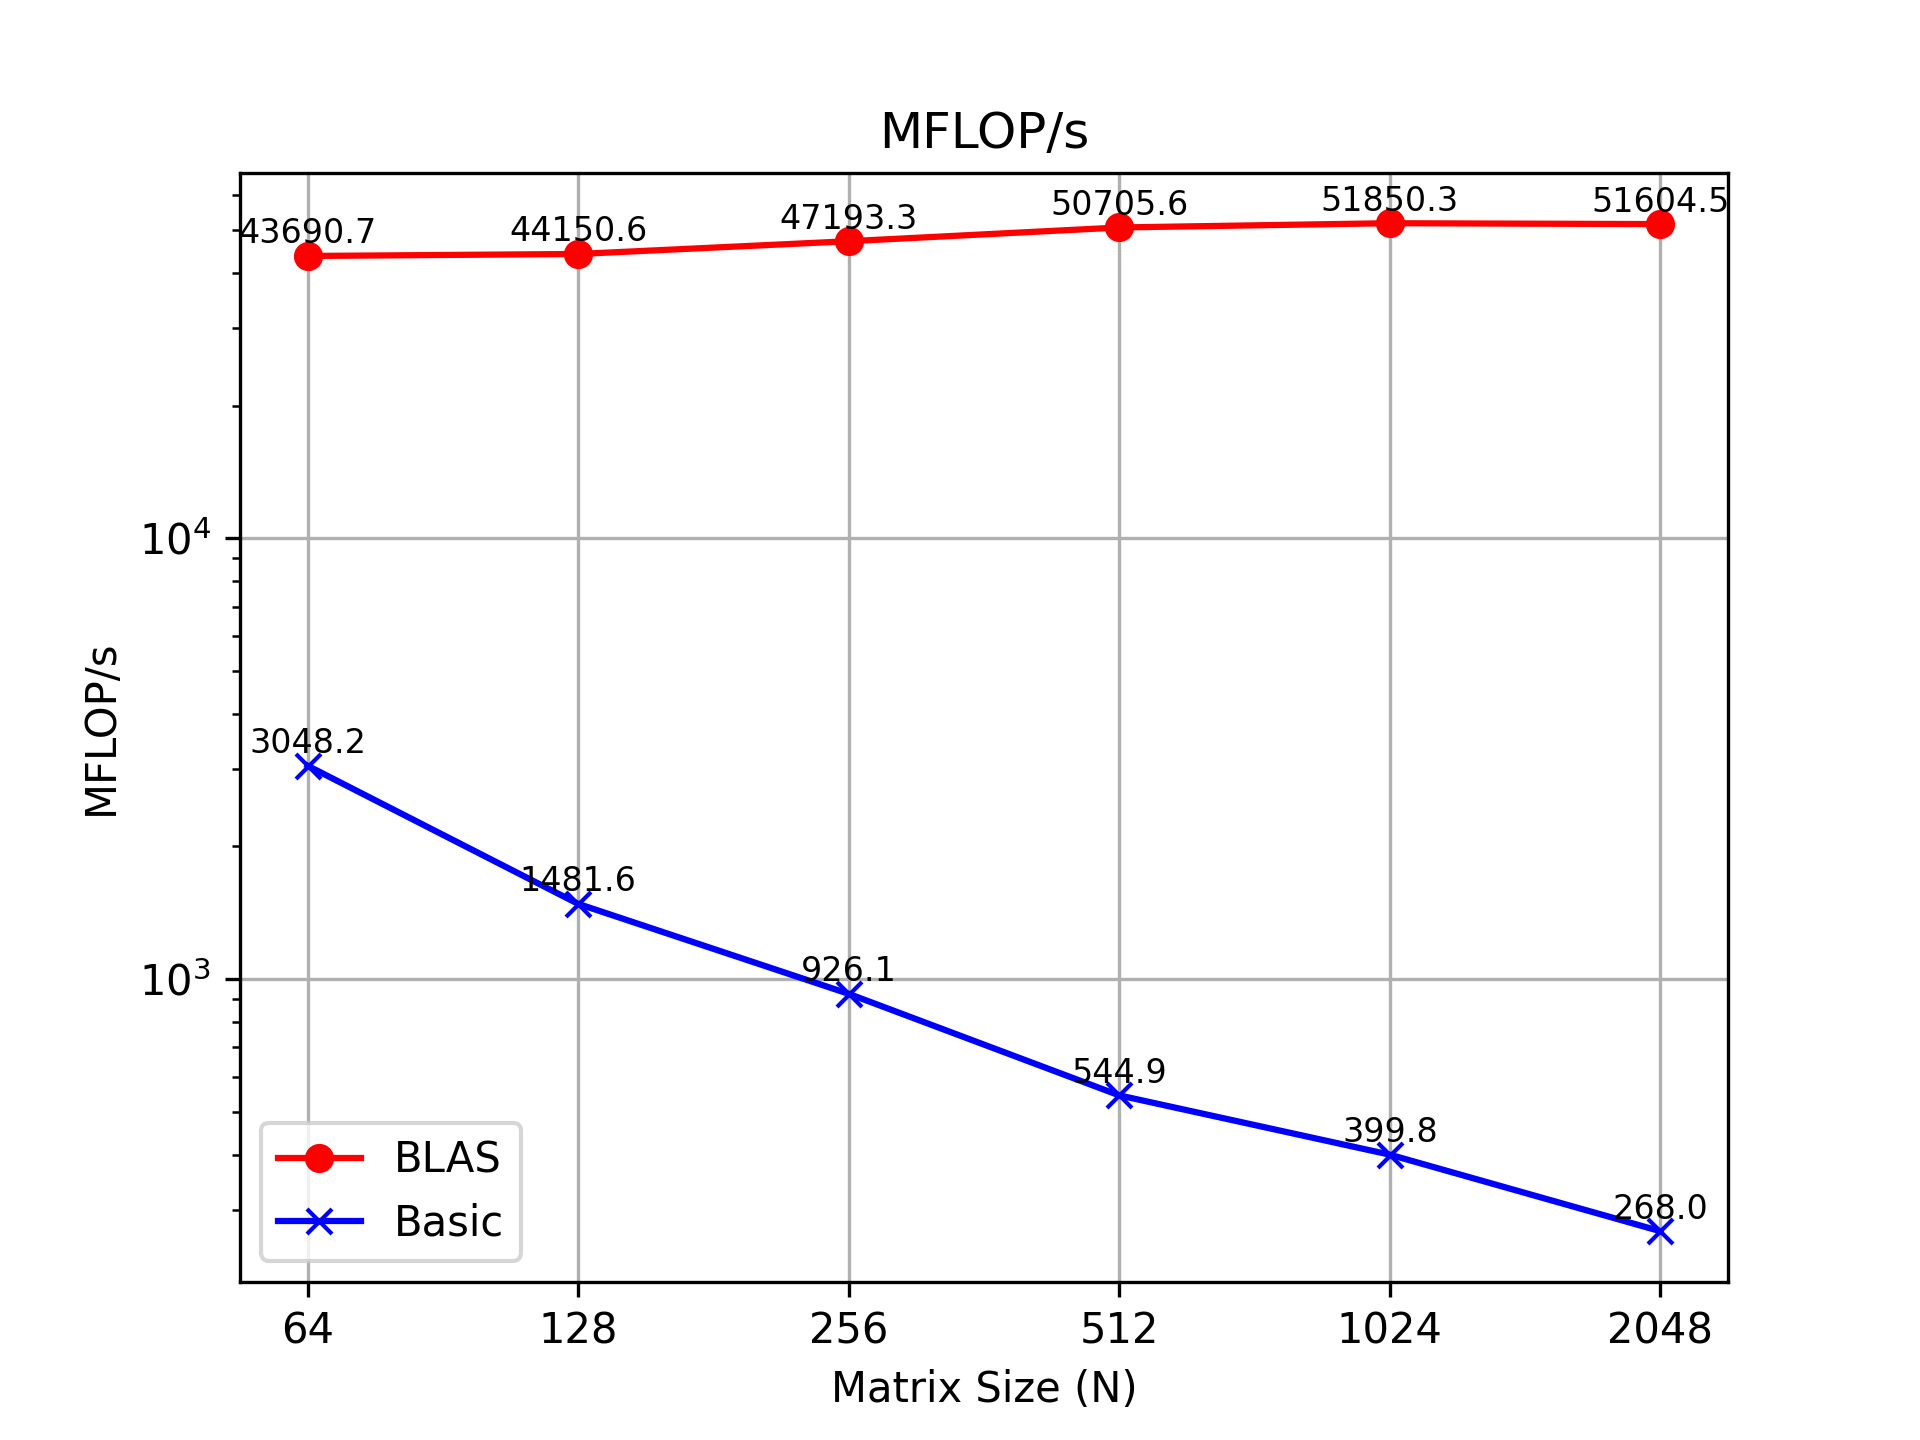
\includegraphics[width=1.0\linewidth]{images/Basic-MM-and-CBLAS_MFLOPs_2nd-run.png}
    \caption{\textbf{MFLOP/s comparison of Basic MM and CBLAS MM for each matrix size when the first run for each size is discarded.} This figure shows a more consistent and gradual increase in performance for CBLAS MM.}
    \label{fig:mflops-Basic-CBLAS-2nd-run}
\end{figure}

\FloatBarrier
\section{Visualizing Blocked Matrix Multiplication}
\label{sec:visualize-bmmco}
The following visualizations represent the process of blocked matrix multiplication using a block size of \(16 \times 16\) for a matrix of size \(64 \times 64\). Each figure corresponds to a specific stage in the computation, illustrating the progression of matrix multiplication. The blocks currently used for computation are highlighted in red, while the green and blue blocks represent memory cache usage (L1 and L2 caches, respectively).

This visualization scripts for blocked matrix multiplication, available at \cite{bmmco_visualization_repo}.

\begin{figure}[htbp]
  \centering
  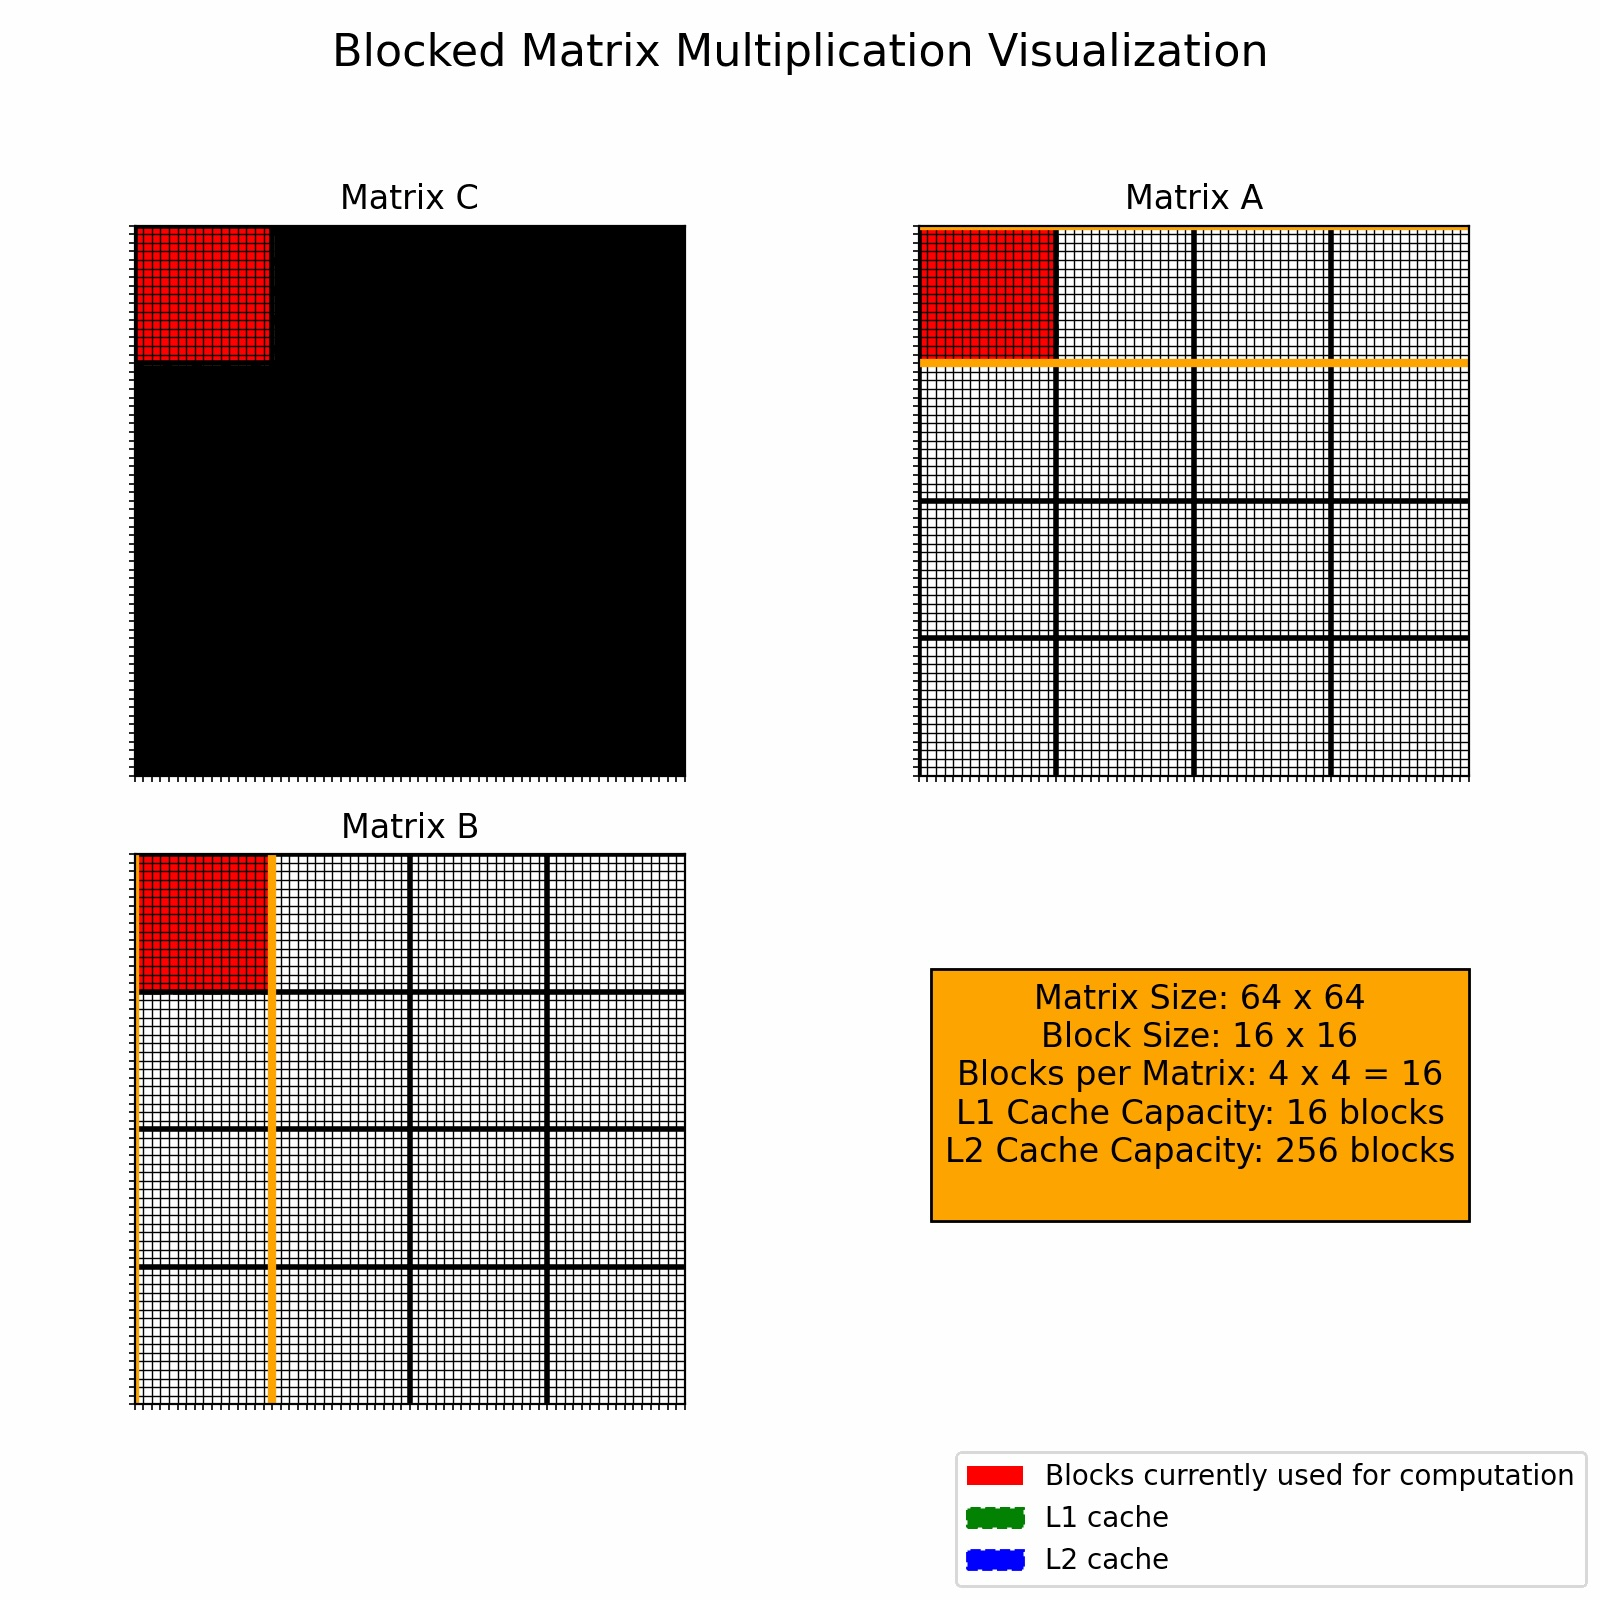
\includegraphics[width=0.8\linewidth]{images/bmmco_animation_0.jpg}
  \caption{\textbf{Blocked matrix multiplication at Frame 0.} Initial frame showing the first block currently used for computation, highlighted in red. The green blocks indicate the sections that fit into the L1 cache, while blue shows the portions stored in L2 cache.}
  \label{fig:frame0}
\end{figure}

\begin{figure}[htbp]
  \centering
  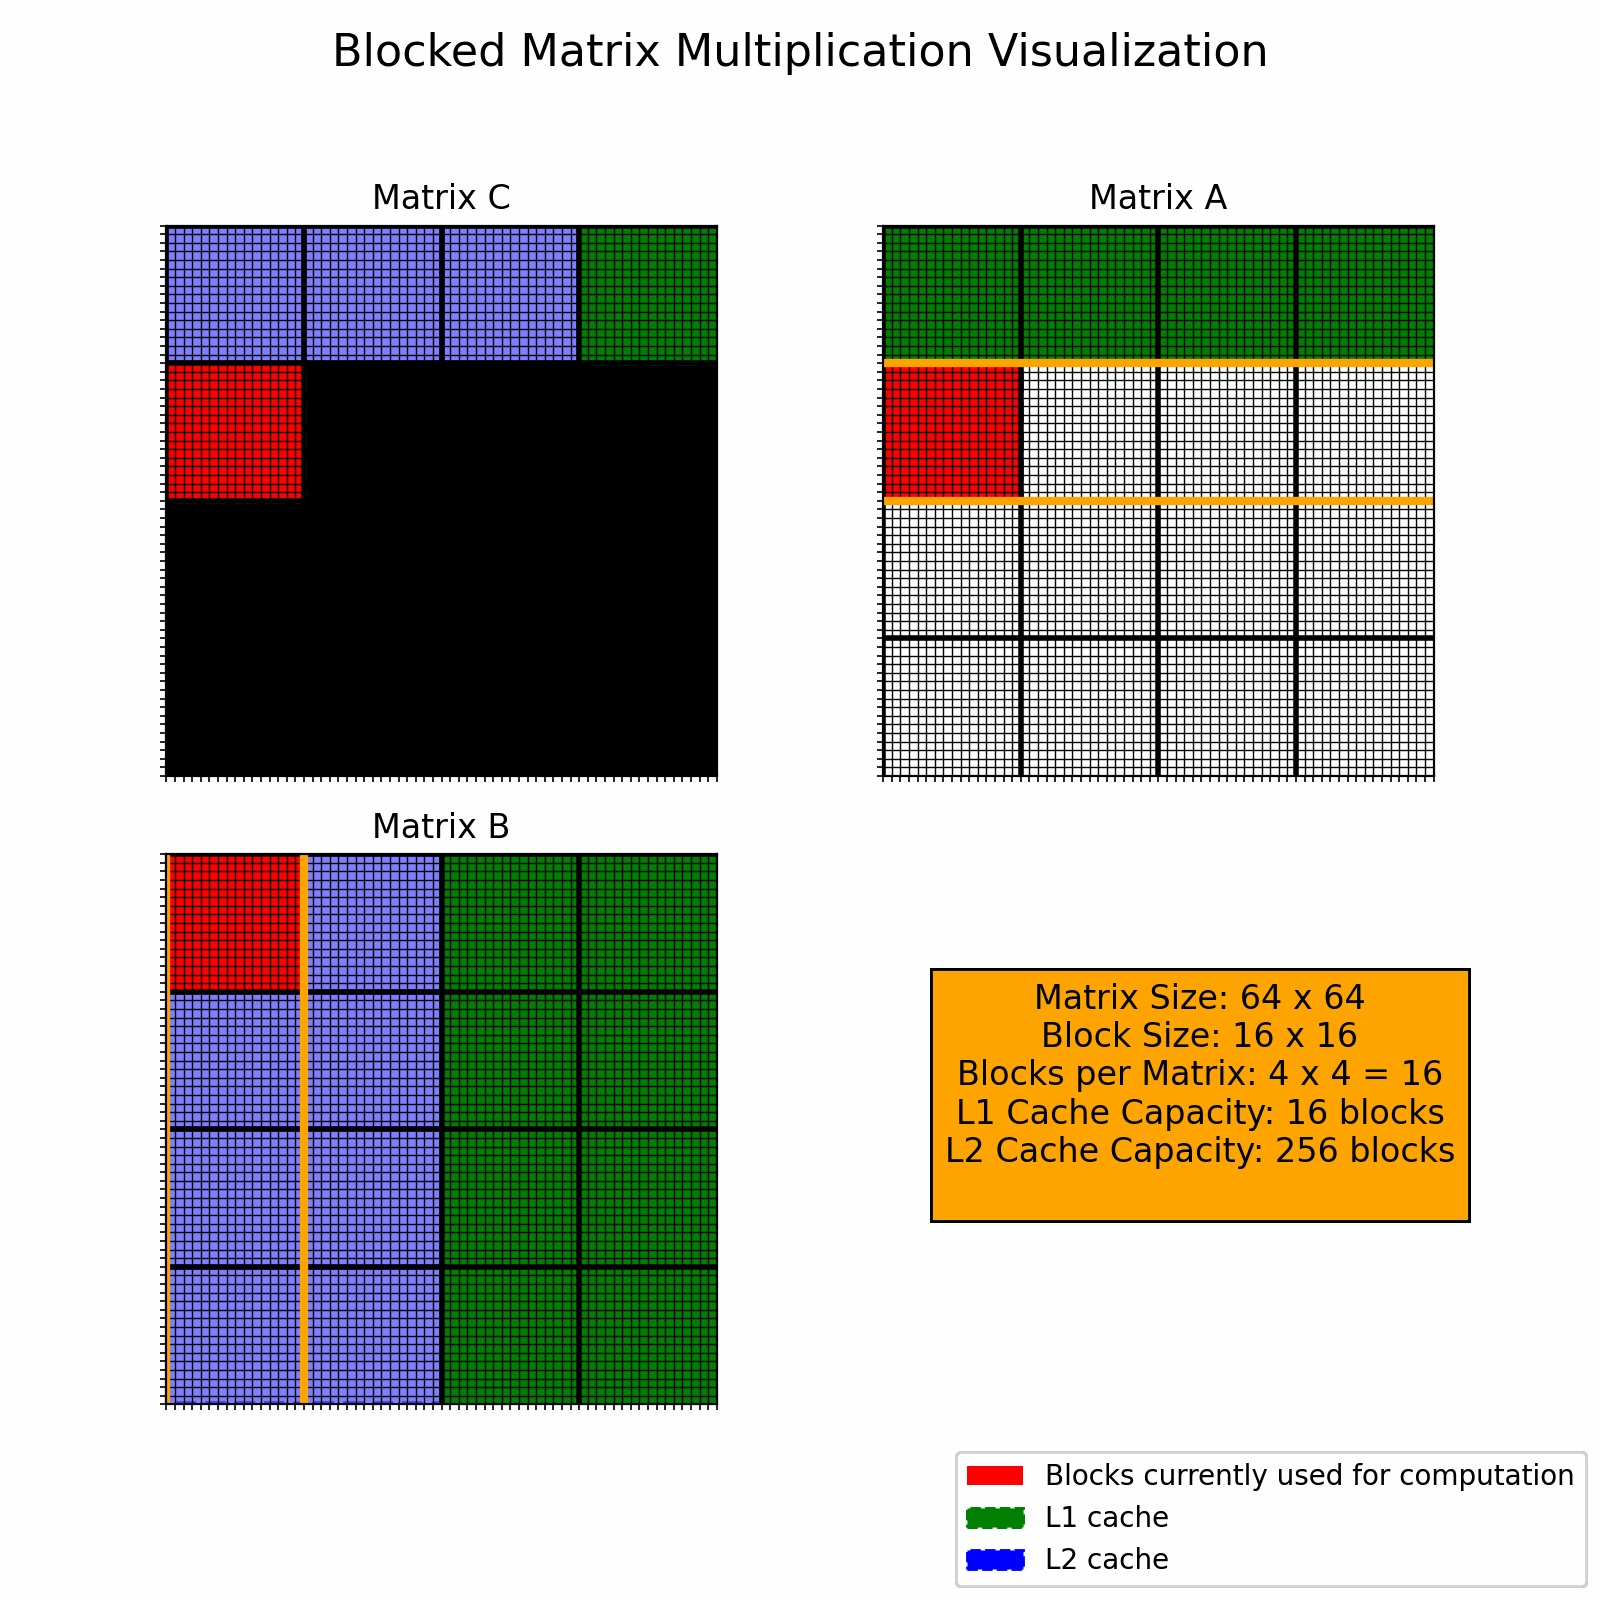
\includegraphics[width=0.8\linewidth]{images/bmmco_animation_17.jpg}
  \caption{\textbf{Blocked matrix multiplication at Frame 17.} In this frame, computation progresses as more blocks are processed. Notice that different blocks of Matrix A and Matrix B are loaded into the L1 cache, and new sections are moved to the L2 cache.}
  \label{fig:frame17}
\end{figure}

\begin{figure}[htbp]
  \centering
  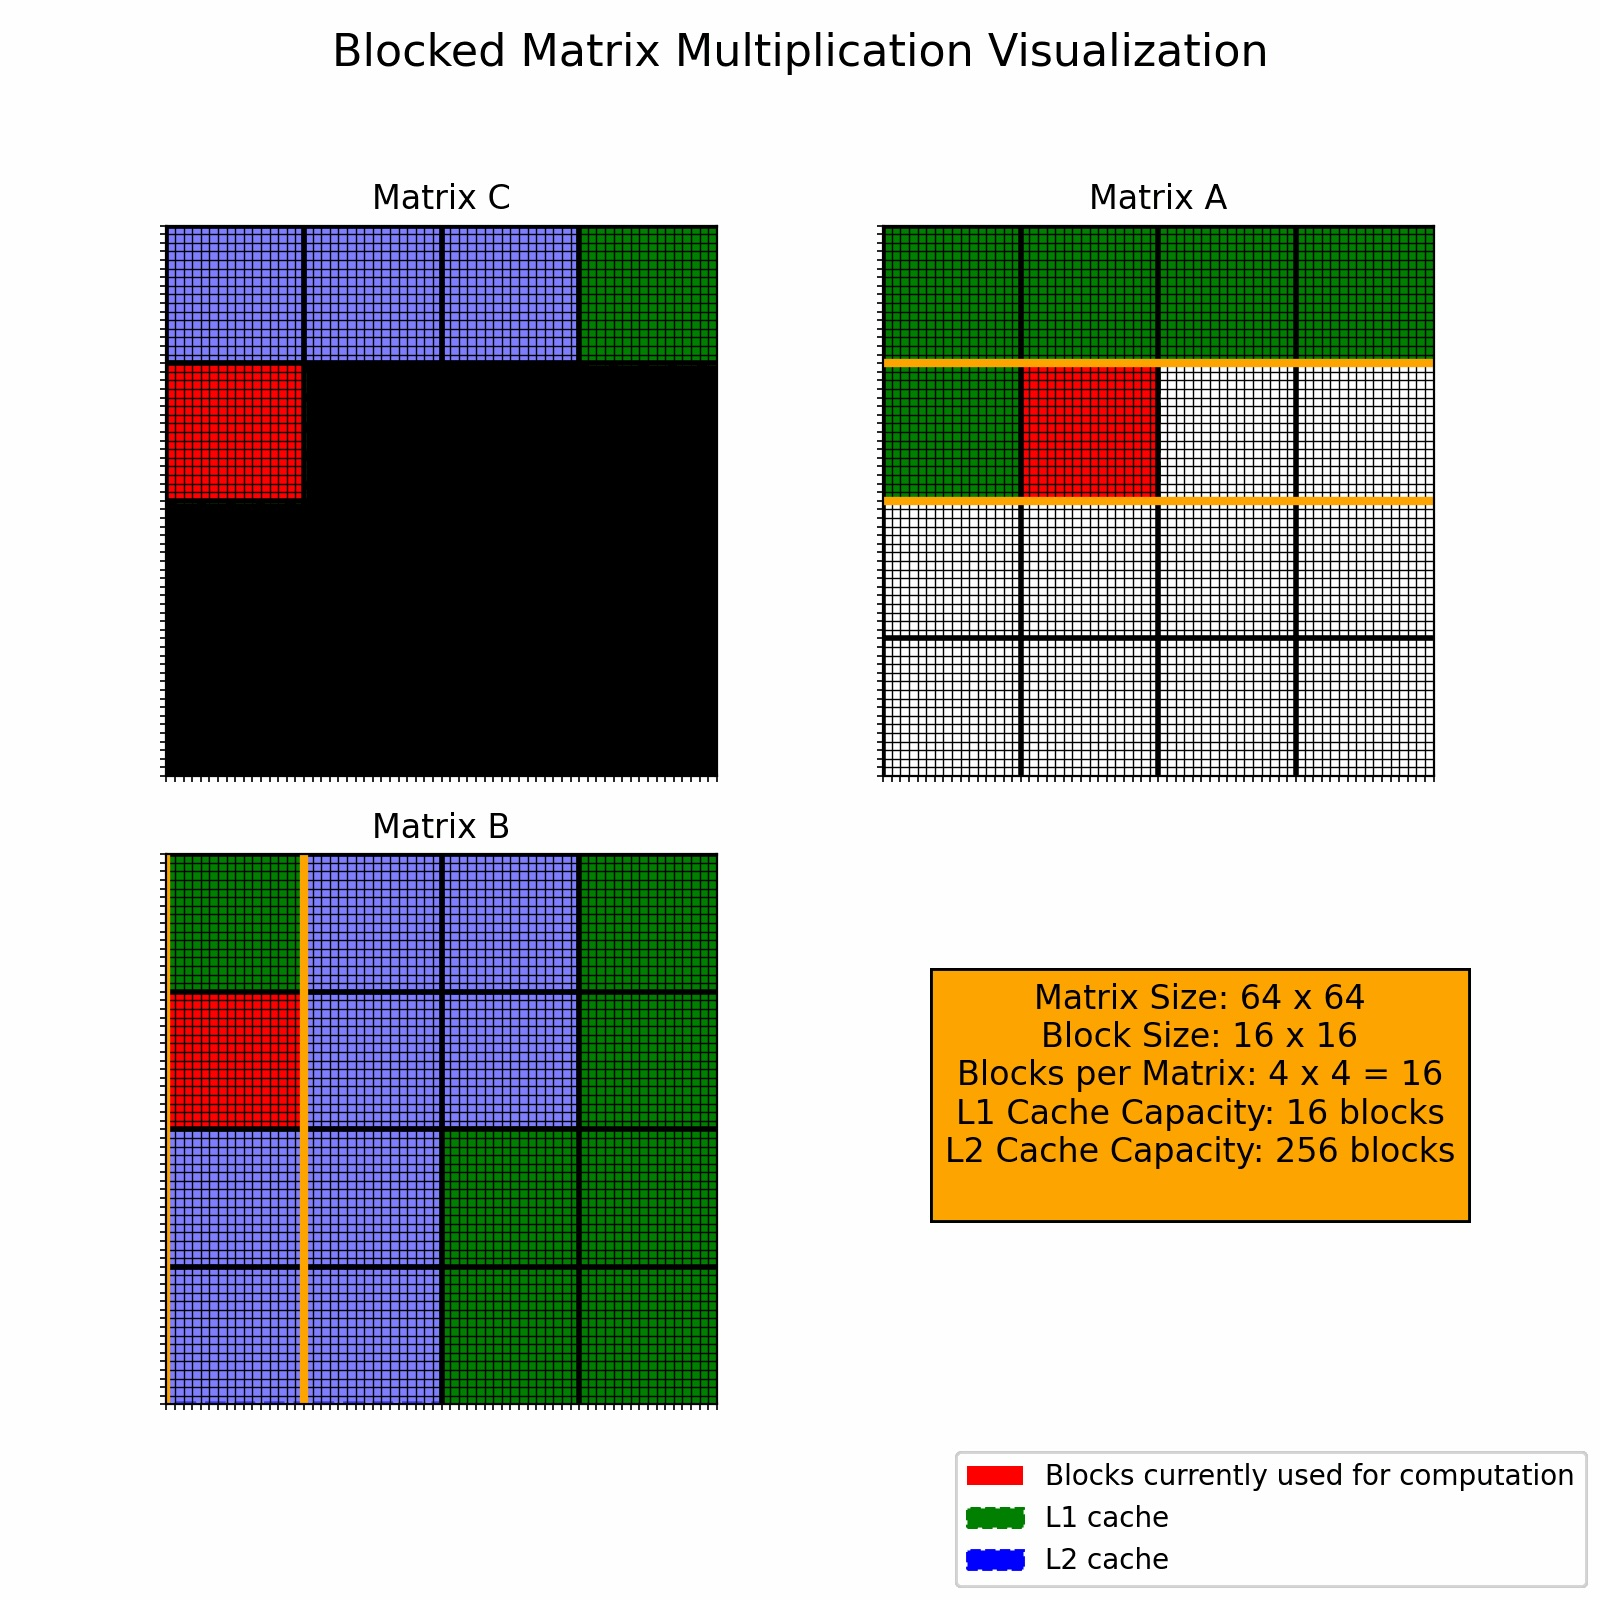
\includegraphics[width=0.8\linewidth]{images/bmmco_animation_18.jpg}
  \caption{\textbf{Blocked matrix multiplication at Frame 18.} The red block in Matrix C is updated as the corresponding blocks from Matrix A and Matrix B are multiplied. L1 cache is utilized to store the blocks of the matrices being multiplied, improving the efficiency of memory access.}
  \label{fig:frame18}
\end{figure}

\begin{figure}[htbp]
  \centering
  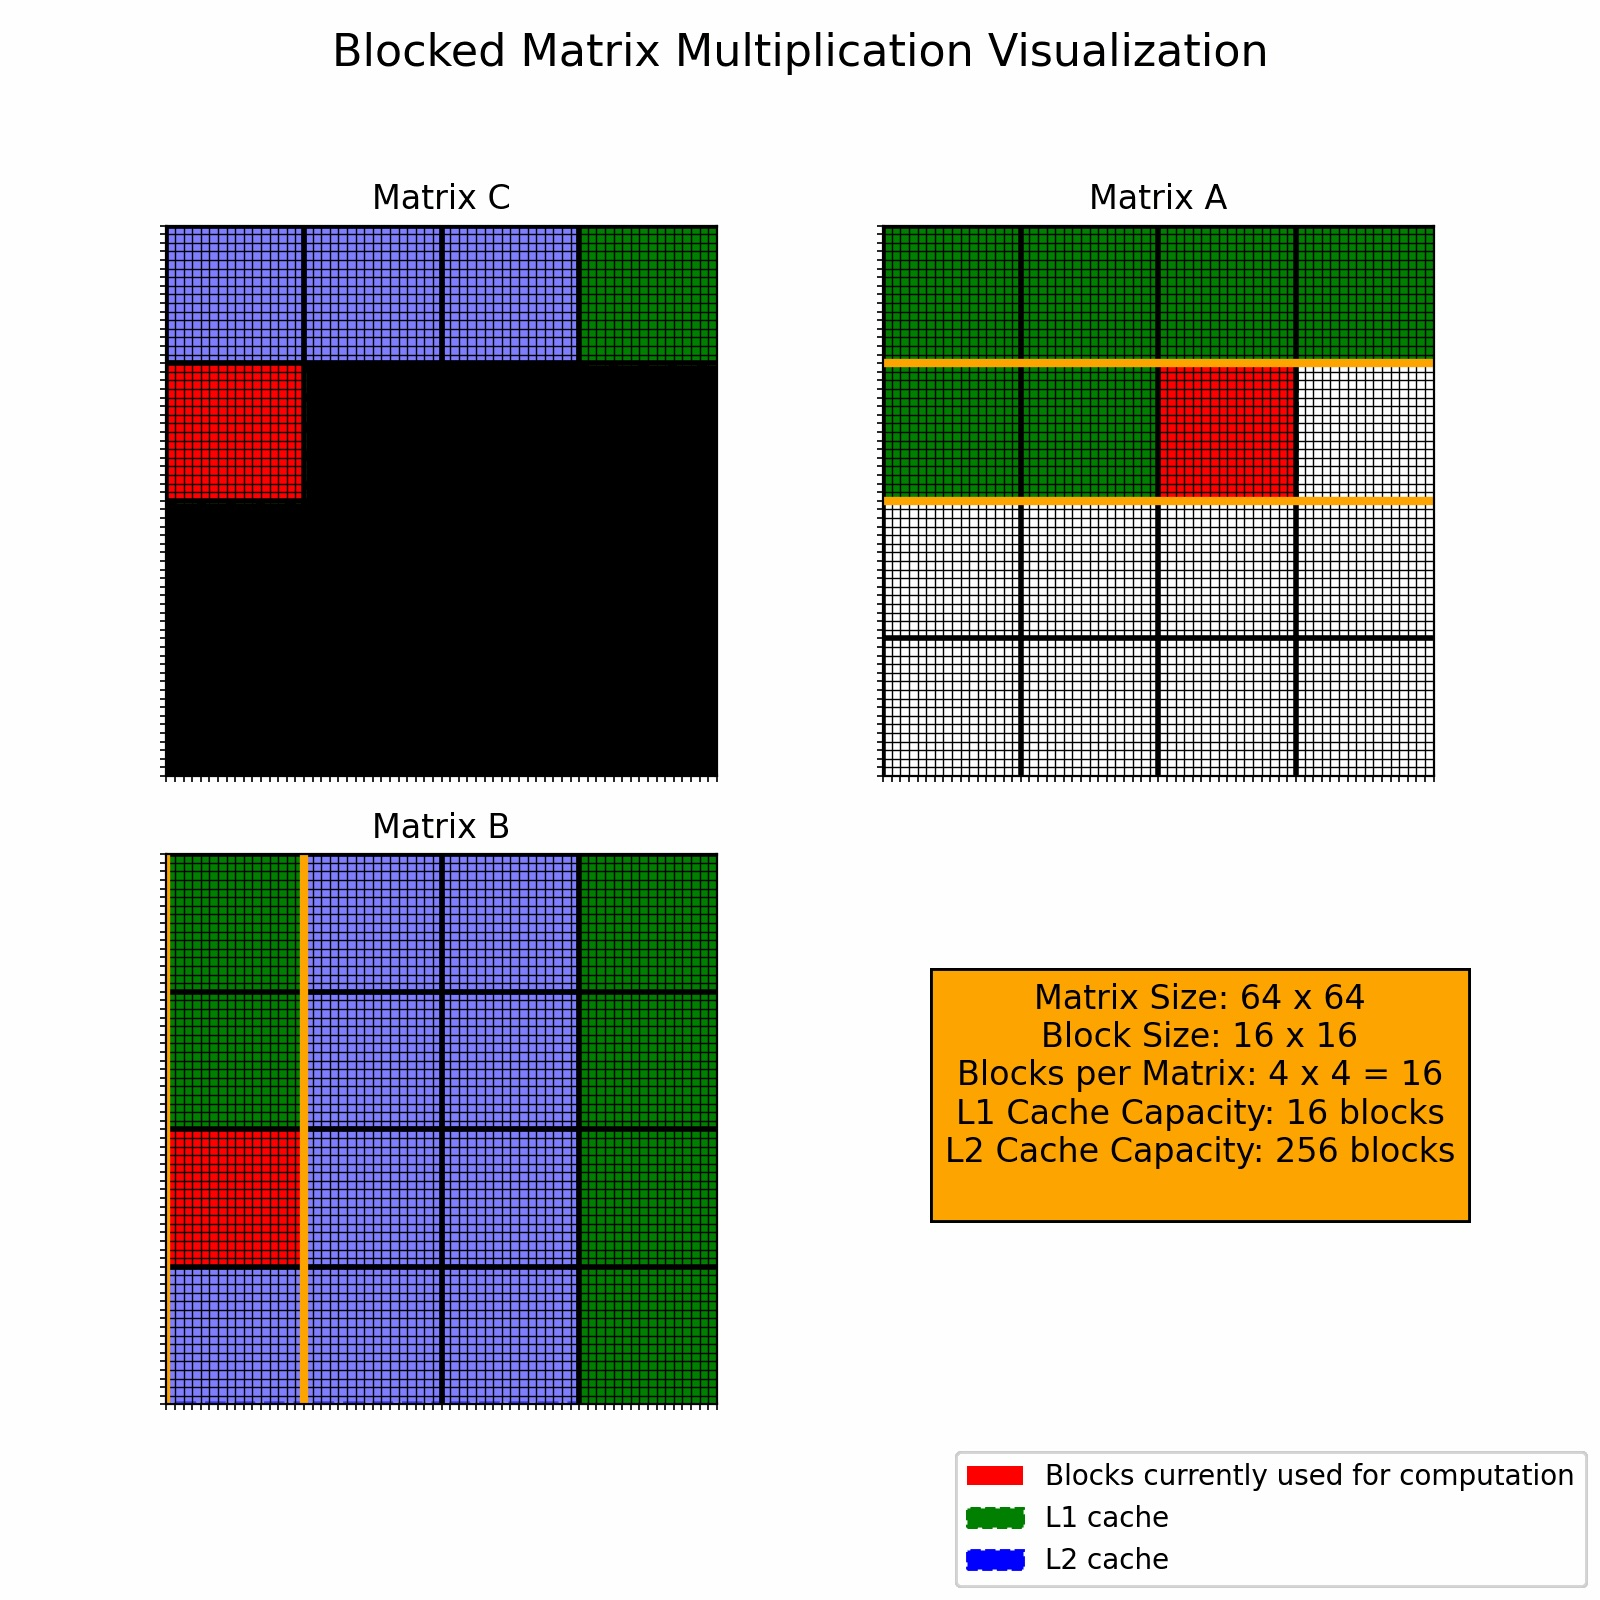
\includegraphics[width=0.8\linewidth]{images/bmmco_animation_19.jpg}
  \caption{\textbf{Blocked matrix multiplication at Frame 19.} The computation moves forward with more blocks being processed. Matrix A continues to slide horizontally, while Matrix B progresses vertically, keeping the working blocks in the L1 cache for quick access.}
  \label{fig:frame19}
\end{figure}

\begin{figure}[htbp]
  \centering
  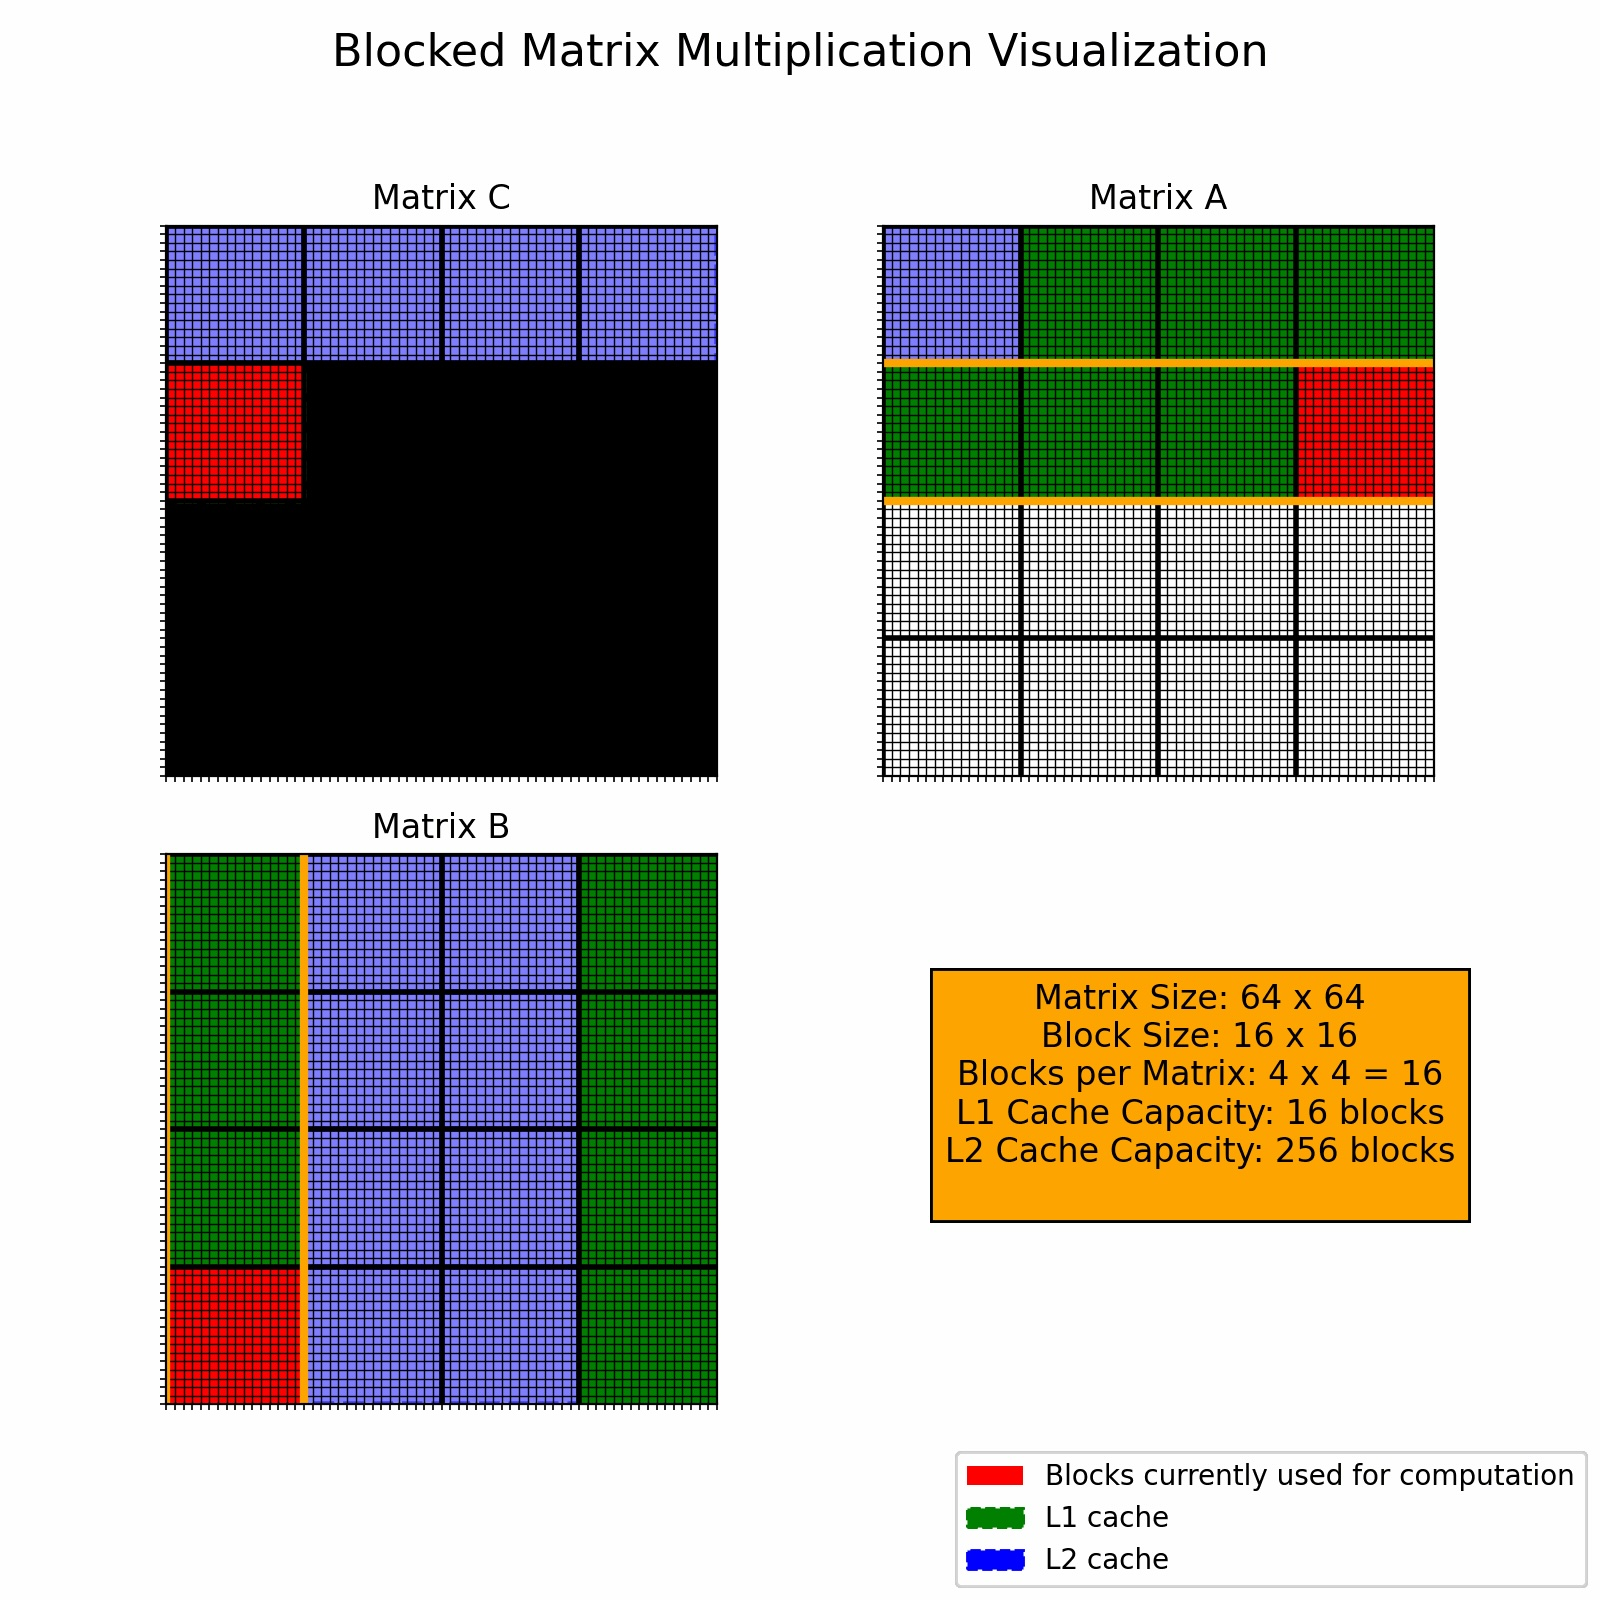
\includegraphics[width=0.8\linewidth]{images/bmmco_animation_20.jpg}
  \caption{\textbf{Blocked matrix multiplication at Frame 20.} The process of multiplying corresponding blocks from Matrix A and Matrix B continues. Matrix C’s red block is updated with new results. By keeping data in the cache, the performance is enhanced due to reduced slow memory access.}
  \label{fig:frame20}
\end{figure}
